\chapter{Literature Review}
\label{ch:lit}
\section{Introduction}

The electrocardiogram (\textbf{ECG}) is one of the most common tests of the
heart, therfore correct interpretation is needed. However, many ECGs are kept as
prints or photographs, that  current software built for digital signals cannot use.
This chapter reviews the work needed to build a system that analyses ECGs directly
from images. The argument is that image-based ECG classifiers have mostly been limited on synthesized images, and that explanations of these results receive little attention. This chapter follows the layout in the following format: Image processing
(Section~\ref{sec:image-processing}) and its function in medical imaging
(Section~\ref{sec:medical-imaging}); the ECG fundamentals (Section~\ref{sec:ecg-fundamentals})
and how an ECG is captured (Section~\ref{sec:ecg-imaging}); Pre-processing
images, the extraction of features from images as well as the detection of waveforms (Sections~\ref{sec:preprocessing}--\ref{sec:waveform}); and relevant algorithms
(Section~\ref{sec:ml-ecg})/existing systems (Section~\ref{sec:existing-systems})
, that outline the gaps addressed by this project.
\section{Digital Image Processing}
\label{sec:image-processing}
An ECG image is a measurement taken via a scanner, so the first point is to discuss what a digital image is. It's a two-dimensional function $f(x,y)$, where $x$ and $y$ are
spatial coordinates and the value of $f$ at each pair is the intensity at that
point, also known as a pixel \cite{gonzalez_digital_2018}. The intensity is the product of the
illumination of the scene and the proportion of light its surface reflects
\cite{stockham_image_1972}: \[f(x,y) = i(x,y)\,r(x,y),\]
where $i$ is the illumination and $r$ is the reflectance, bounded by 0 (total
absorption) and 1 (total reflection). As $i$ can change whilst $r$ stays the
same, one object can look different under different lighting. In the same way, a single \textbf{ECG}
trace can form many different images. Signals like \textbf{ECGs} are often continuous. As computers have insufficient memory to store continuous
functions, images are instead digitised by sampling, which divides the image into a grid
of pixels, and quantisation, which rounds each value to one of a finite number of
intensity levels. A higher sample rate produces a higher resolution. The quantisation step is irreversible, as rounding up or down discards any difference (albeit at 8 bits per pixel
this loss is rarely visible).\cite{gonzalez_digital_2018}.

Image enhancement makes an image more suitable for a task, whereas image restoration fixes found degradations. One technique that is used is \textbf{Histogram equalisation (HE)}, which spreads pixel values across
the full intensity range. Whilst this increases contrast, the drawback is it handles local detail poorly. An updated version named \textbf{contrast-limited adaptive histogram equalisation (CLAHE)} instead works on local
regions and limits the amount of noise \cite{zuiderveld_contrast_1994}. Once  contrast is adjusted, noise must be cleaned up to limit the amount of artefacts on an image. Most commonly, spatial filters are used, where it looks at each pixel and its immediate neighbours. Spatial
filters often have specific drawbacks: For example, gaussian filters reduce random noise, but blur edges
\cite{gonzalez_digital_2018}; median filters remove "salt and pepper" noise, whilst preserving
edges better; and bilateral filtering smooths flat regions (like the grid) whilst keeping any vertices sharp \cite{verma_ali_2013}. In contrast, frequency-domain methods often work on a transformed images. Namely, the
inverse Fourier Transform (FT) describes an image as a sum of patterns at different frequencies,
\begin{equation}
  f(x,y) = \frac{1}{MN}\sum_{u=0}^{M-1}\sum_{v=0}^{N-1}
           F(u,v)\,e^{\,j2\pi\left(\frac{ux}{M}+\frac{vy}{N}\right)}
  \label{eq:inv-fourier}
\end{equation}
so regular repeating patterns, which appear as sharp peaks, can be removed with a
notch filter. Similarly, \textbf{Homomorphic filtering (HF)} takes the logarithm of the image and turns the product $i\,r$ into a sum, so that $i$ (low frequency) can be
suppressed and $r$ (high frequency) boosted. As a result, \textbf{HF} suits uneven lighting, but can amplify noise. On the other hand, \textbf{Wavelet transforms (WT)} split an image into components at
several scales whilst keeping their position, which suits noise removal
\cite{lepcha_deep_2023}. Combining \textbf{HF} and \textbf{WT} is the technique to remove noise and keep detail. We must consider that removing noise can distort real
detail, and no single method suits every image, so the choice depends on the
degradation and the task \cite{qi_comprehensive_2022}.

To extract the ECG from an image, segmentation divides a cleaned image into meaningful regions. Some examples are to use thresholding,
which separates foreground from background with an intensity cut-off chosen manually or
automatically \cite{otsu_threshold_1979} (Figure~\ref{fig:otsu-dermatoscopic}), or edge
detection \cite{canny_computational_1986}. In conjuntion, morphological operations like opening and
closing clean up the result \cite{gonzalez_digital_2018}.

\begin{figure}[ht]
  \centering
  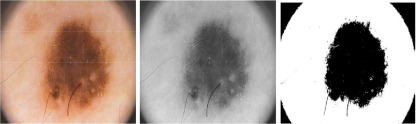
\includegraphics[width=0.38\linewidth]{images/OtsuSegmentation.jpg}
  \caption[Otsu segmentation of a dermatoscopic image]{Example of Otsu
    segmentation of a dermatoscopic image, obtained from the \(PH^2\) dataset.
    Reproduced from \cite{mendonca_ph_2013}.}
  \label{fig:otsu-dermatoscopic}
\end{figure}

To interpret an image, the most popular approach is a \textbf{convolutional neural
network (CNN)}, which learns features from labelled examples by applying small
filters learned during training\cite{lecun_gradient_1998}. Stacked layers build up from simple edges to complex patterns, so features need not be designed by hand, although a large dataset is needed. Each stage has its trade-offs, from  removing unwanted variation against
preserving detail, and these trade-offs matter more when images support medical
decisions.
\section{Medical Image Processing}
\label{sec:medical-imaging}

Medical images follow the same image processing as other types, but must preserve as much anatomical detail as possible. Noise is the main threat:
\textcite{prasad_systematic_2023} state that it can degrade diagnostic quality significantly by blurring borders, reducing contrast and obscuring important detail. A common noise model is \textbf{Gaussian noise (GN)}, which is added independently to each pixel,
\begin{equation}
  I(x,y) = J(x,y) + N(x,y),
  \label{eq:gaussian-noise}
\end{equation}
where $I$ is the noisy image, $J$ is the original and $N$ is drawn from a normal
distribution with mean 0 and variance $\sigma^2$, so a larger $\sigma^2$ means
stronger noise. %add to glossary

The general methods of Section~\ref{sec:image-processing} have been adapted for medical use, but each involved a trade-off. Adaptive \textbf{HE} was developed for medical image displays \cite{pizer_adaptive_1987}, yet even its contrast-limited form
needs the clip limit to be tuned, and in addition, averaging filters suppress noise whilst blurring the
edges that carry important diagnostics. Whether an enhancement helps therefore
depends on the task. In medical imaging, quality is best defined by how well an
observer can perform a specific task, not by how the image looks
\cite{barrett_foundations_2004}. A sharper image does not necessarily lead to better decision making, and enhancement that suits a human viewer may not help a classifier.

As hand-designed methods depend on assumptions about the image, learned methods
have largely replaced them. A survey of over 300 studies found \textbf{CNN}s  are used
across the medical imaging field, including cardiac applications \cite{litjens_survey_2017}.
Often, \textbf{CNN's} bring their own issues. For example, labelled data is expensive and abnormal cases are rare, and performance may not carry over to new data; \textcite{zech_variable_2018} found
that networks for detecting pneumonia in chest radiographs performed differently
across three hospital systems. In addition, models may also rely on shortcuts that correlate with the label instead of the features that matter \cite{geirhos_shortcut_2020}, and as predictions may influence patient decisions, systems must explain their output, like with Grad-CAM \cite{selvaraju_gradcam_2017}, or report calibrated
confidence \cite{guo_calibration_2017}. So in this project, preprocessing will be judged by its effect on classification and not by appearance. Also, he gap between rendered training images and real
test images is a generalisation problem, so the model may pick up features of the rendering that real images do not have.

\section{ECG Fundamentals}
\label{sec:ecg-fundamentals}

The \textbf{ECG} is an electrical tracing of the heart, recorded non-invasively
from the surface of the body \cite{sattar_electrocardiogram_2023}. It shows how the impulse that triggers each heartbeat spreads through the heart, so it is well suited
to detecting problems of rhythm and conduction. Each heartbeat produces a repeating
sequence of deflections (Figure~\ref{fig:ecg-beat}): the P wave reflects activation of the atria, the QRS complex shows activation of the ventricles, and the T wave shows their
recovery. The intervals between these features carry diagnostic information: the PR interval reflects the delay as the impulse passes from the atria to the ventricles, the QRS duration how quickly the ventricles are activated, and the QT interval spans
ventricular activation and recovery. Abnormalities are defined by changes to these features, so a model working from an image must find them and judge their shape and
spacing.

\begin{figure}[ht]
  \centering
  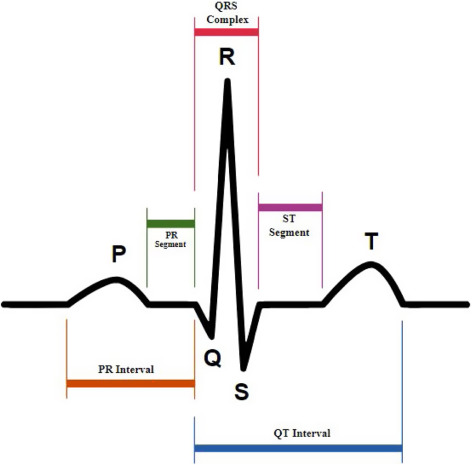
\includegraphics[width=0.35\linewidth]{images/LabelledHeartbeat.jpg}
  \caption[A single PQRST wave]{A single heartbeat, showing the P wave, QRS complex,
    T wave and main intervals. Generated by the author from
    \cite{Mazomenos_ECG_2012}.}
  \label{fig:ecg-beat}
\end{figure}

A standard resting \textbf{ECG} records twelve leads: six limb leads and six chest
leads \cite{sattar_electrocardiogram_2023}. Each lead views the same heartbeat from a
different orientation, so an issue in one region of the heart often appears in only some
leads. A regular page cannot fit twelve full-length traces, so the printout cuts each into a
short piece and arranges them on a $3\times4$ grid \cite{ashley_conquering_2004}
(Figure~\ref{fig:ecg-grid}). Thus, a single image contains twelve traces, and a
classifier must learn which leads matter for which condition. On the grid, the distance $x$ along the paper and the deflection $y$ are converted to time and voltage by $t = x/v$ and
$V = y/g$, where $v$ is the paper speed and $g$ the gain (25\,mm/s and 10\,mm/mV as
standard \cite{sattar_electrocardiogram_2023}). Clinicians read rate and intervals by
counting squares; for example, the heart rate follows from the RR interval 
(\(\mathrm{HR} = 60/\mathrm{RR} = 300/N\))
where RR is the time in seconds between successive R peaks and $N$ is the number of
large squares between them. Timing and amplitude can thus only be read from an image if
the grid calibration is known, so skewing, cropping, resizing or photographing the page
all distort it.

\begin{figure}[ht]
  \centering
  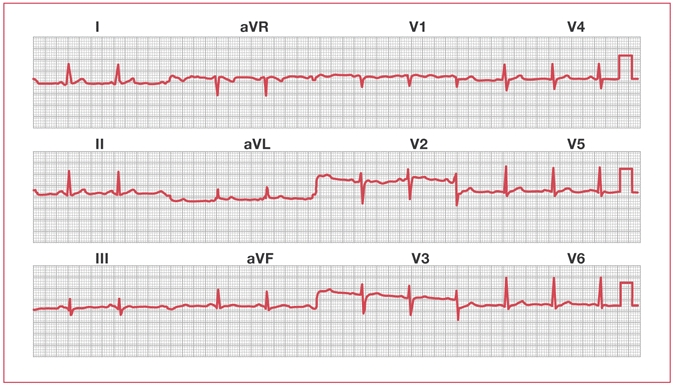
\includegraphics[width=0.4\linewidth]{images/ECGGrid.jpg}
  \caption[An ECG paper trace]{A single trace, showing a $3\times4$ grid of leads
    \cite{ashley_conquering_2004}.}
  \label{fig:ecg-grid}
\end{figure}

Abnormalities are grouped by what they affect. Abnormal heart
rates and rhythms are known as arrhythmias \cite{nhs_heart_2018}; they include atrial
fibrillation and atrial flutter % put in glossary mate 
, where beats are irregularly spaced and clear P waves are absent
\cite{van_gelder_2024_2024}, and atrial flutter, which shows a regular saw-tooth
pattern in the inferior leads \cite{cosio_atrial_2017}. Conduction disturbances such as
\textbf{bundle branch blocks (BBB)} usually widen the QRS complex \cite{scherbak_left_2024},
\textbf{myocardial infarction (MI)} and other ischaemic changes often alter the ST segment and T wave
in the leads facing the affected region, and hypertrophy of the heart's chambers is
associated with changes in amplitude \cite{channer_myocardial_2002}. Some of these
abrnormalities depend on the shape of the trace, whereas others depend on timing and regularity,
which in an image depends on the grid scale.

Currently, datasets have encoded these findings as "labels", like the PTB-XL dataset, contains 21,800 ten-second twelve-lead \textbf{ECG}s from about 19,000 patients. They are annotated by cardiologists, with diagnostic labels grouped into five superclasses (normal, \textbf{MI}, ST/T change,
conduction disturbance and hypertrophy) plus form and rhythm statements. A single record can carry several labels \cite{wagner_ptbxl_2020}. It provides signal data, not real images. For real images, a dataset from UMT \cite{khan_ecg_2021} contains real images with various levels of degradation. These
fundamentals define the classes this project will detect and the two kinds of
information the classifier must use: the shape of each beat, and the timing between beats.

\section{ECG Imaging and Digitisation}
\label{sec:ecg-imaging}

Although ECGs are recorded digitally, they are often scanned, photographed, or printed. Such images cannot be used directly by software that expects
signalled data \cite{shivashankara_ecg-image-kit_2024}. Physical ECGs also vary widely. The
ECG-Image-Database, for example, contains printed ECGs that were scanned or photographed under different lighting conditions, artifacts on the image and camera angles \cite{reyna_ecg-image-database_2024}. This is the illumination and reflectance
effect of Section~\ref{sec:image-processing} at work, and its consequence was reported in practice: \textcite{gliner_domain_2023} needed to adaptation to the domain to retrain a model from scans to captured images. To further add, image resolution also limits how accurately the trace can be read, therefore it directly limits the timing measurements that some classes depend on.

There are two approaches that address the problem. Digitisation reconstructs the  signal
from the image so that signal-based methods can be applied. Whilst this produces
measurable intervals, it needs several steps (locating the grid, separating the leads
and tracing each waveform). Additionally, a single error at any step will carry through to the
reconstructed signal. The George B.\ Moody PhysioNet Challenge 2024, for example,
evaluated digitisation by the \textbf{signal-to-noise ratio (SNR)} of the recovered
signal \cite{physionet_challenge_2024}. The other option is to classify the image directly (Section~\ref{sec:ml-ecg}), which avoids reconstruction, but the model must then learn the timing from pixels. This means its results depend on how the images were produced, which is the generalisation problem of Section~\ref{sec:medical-imaging}.Data for this approach have been taken from 2 sources. \textit{ECG-Image-Kit} generates
synthesized ECG images from real signals, with the addition of artefacts
\cite{shivashankara_ecg-image-kit_2024}. The \textit{ECG-Image-Database} provides about 36,000
images by combining records from PTB-XL and Emory Healthcare that were printed, degraded, % mention Emory Healthcare
and then scanned or photographed \cite{reyna_ecg-image-database_2024}. This project
analyses ECG images directly and avoids a the step to digitising signals. Instead, it trains on images
rendered from PTB-XL and tests on real-world images, so that the effect of real imaging
conditions can be measured.

\section{Pre-processing and Noise Removal}
\label{sec:preprocessing}

Preprocessing corrects problems introduced during printing and capture, using the
methods of Section~\ref{sec:image-processing},matched to faults that occur in \textbf{ECG}
images. Nevertheless, each choice carries a risk. For instance, uneven lighting and shadows can be reduced with \textbf{CLAHE}
\cite{pizer_adaptive_1987,zuiderveld_contrast_1994} or \textbf{HF}
\cite{stockham_image_1972}, but at the cost of increased noise. Noise and specks
(Equation~\ref{eq:gaussian-noise}) can be reduced with median filtering, bilateral
filtering \cite{tomasi_bilateral_1998} or non-local means \cite{buades_non-local_2005},
, but they can flatten thin peaks. The printed grid can be removed by colour
segmentation or notch filtering \cite{gonzalez_digital_2018}, but it would struggle with faded
or monochrome prints, and rotation can be corrected by line detection, but it also cannot fullyundo the perspective distortion of a photograph.

The grid especially needs particular care as it is both noise and information: not only it can cross the
trace and can confuse a classifier, but it is also the only record of the time and voltage scale (Section~\ref{sec:ecg-fundamentals}). This means removing it without noting the
scale first would remove factors influencing the measurements. The trace is also really thin, so
smoothing or enhancement can actually remove P waves and sharp QRS peaks that are only a few
pixels wide. In addition, it is not certain that preprocessing actually helps a \textbf{CNN} at all, as there is a possibility that a
network trained on varied, images may learn to cope with them. Therefore, preprocessing is a design choice, judged by its effect on classification performance and not by how the image looks.

\section{Feature Extraction}
\label{sec:features}

Before deep learning networks existed, automated \textbf{ECG} analysis relied on hand-designed features. Once the
rhythm were located, quantities such as interval lengths and wave amplitudes were measured and passed to a classical classifier, as in the heartbeat classification of\textcite{de_chazal_automatic_2004}, which combined morphology and interval features.
Such features have a clear clinical meaning, which makes the model easier to explain, and
timing features are especially useful for rhythm. The regularity of the RR intervals, for
example, separates a regular rhythm from an irregular one (such as atrial fibrillation). The
alternative is learned features, where a \textbf{CNN} builds its features directly from the pixels
\cite{lecun_deep_2015}. This indicates that no one has to decide in advance what to measure.
Hand-designed features are easy to interpret, but depend on every previous step succeeding, as a missed beat or a broken trace corrupts every feature that follows. Learned
features avoid this dependency, but also are harder to explain and need a large labelled
dataset to be trained on.

This project uses both. A \textbf{CNN} learns shape-based features from the image, which suits the diagnostic superclasses.The rhythm classes depend on the spacing between beats, which a model can only judge correctly
if the scale is consistent across images. Measured timing features from the
next paragprah (Section~\ref{sec:waveform}) address this.

\section{Waveform Detection}
\label{sec:waveform}

Waveform detection finds the parts of the \textbf{ECG} that features are measured from. In digital
signals, this usually means locating the QRS complex. The Pan--Tompkins algorithm does so in real time by band-pass filtering and differentiating the signal, squaring it,window-smoothing, and applying adaptive thresholds \cite{pan_real-time_1985}. For an image, the first task is finding the trace itself. Some published work binarise the image,
remove the grid and text, repair gaps in the trace and locate each lead, using a Hough transform to find the grid lines or lead baselines
\cite{wu_automated_2022}. Each column of the isolated trace is then
reduced to one value, for example, the median vertical position of the trace pixels \cite{wu_automated_2022}. This is converted to time and voltage using the grid scale, after which peaks can be detected as in the signal case.

Explicit detection gives measurable intervals and a rate that a clinician can check, and
it can be very accurate. \textcite{randazzo_development_2022} reported an average correlation of
0.94 with reference signals on images from 16 subjects, and \textcite{wu_automated_2022}
 found about 0.99 on standard layouts, once images with overlapping leads were excluded. Conversely, it is also
fragile. The correlation of \textcite{wu_automated_2022} fell to about 0.96 on printed and
rescanned \textbf{ECGs}, whilst \textcite{wadehn_ecg_2024} scored a
\textbf{SNR} of $-2.44$\,dB on 100 rendered PTB-XL images,which indicates that background noise dominates the cardiac signal. This means that it can degrade the waveform, and even a missed or false peak changes the RR intervals and every timing feature
that follows, so errors made at this step carry through to the prediction. This project therefore
uses waveform detection to find the trace and the beats, whilst supplying  the timing features
alongside the learned image features. It will evaluate the detection step on real-world images
and not only on rendered ones.

\section{AI/ML Algorithms for ECG Analysis}
\label{sec:ml-ecg}

Deep learning has largely replaced feature-based methods for \textbf{ECG}classification
(Table~\ref{tab:ecg-studies}). On signals, networks reached cardiologist-level performance on single-lead rhythm classification \cite{hannun_cardiologist_2019}. They also outperformed cardiology residents on 12-lead abnormalities \cite{ribeiro_automatic_2020}. Finally, a PTB-XL
benchmark found convolutional architectures, like ResNet- and Inception-based ones,
performed best \cite{strodthoff_deep_2021}. On the contrary, image-based work is newer.
\textcite{sangha_automated_2022} trained a \textbf{CNN} on images generated from signals
and tested it on various forms of external ECGs, \textcite{gliner_domain_2023} used
domain adaptation to transfer a model to phone-captured images, and
\textcite{wang_pipeline_2025} fine-tuned a ConvNeXt backbone first on synthetic and
external images. Because labelled \textbf{ECG} images are limited, such work relies on transfer
learning, in which networks such as ResNet \cite{he_deep_2016}, pretrained on natural
images, learn general features that transfer to new tasks
\cite{yosinski_transfer_2014}.

\begin{table}[ht]
  \centering
  \footnotesize
  \caption{Key studies in deep learning for ECG classification.}
  \label{tab:ecg-studies}
  \begin{tabular}{@{}p{0.13\linewidth} p{0.27\linewidth} p{0.25\linewidth} p{0.25\linewidth}@{}}
    \toprule
    \textbf{Study} & \textbf{Input and data} & \textbf{Reported result} &
      \textbf{Limitation for this project} \\
    \midrule
    \textcite{hannun_cardiologist_2019} &
      Single-lead signals; 91,232 ECGs, 53,549 patients &
      12 rhythm classes; F1 0.837 vs.\ 0.780 for cardiologists &
      Single lead; signals, not images \\
    \textcite{ribeiro_automatic_2020} &
      12-lead signals; over two million exams &
      Six abnormalities; F1 above 80\%, specificity above 99\% &
      Signals, not images \\
    \textcite{strodthoff_deep_2021} &
      12-lead signals, PTB-XL &
      Convolutional models performed best &
      Signals; hidden weakness in subclasses \\
    \textcite{sangha_automated_2022} &
      Images generated from signals; printed ECGs to test &
      Strong performance on held-out, external and printed ECGs (0.98 AUROC average) &
      Training images are generated from signals \\
    \textcite{gliner_domain_2023} &
      79,226 scanned labelled ECGs plus unlabelled phone-captured frames &
      Average AUROC of 0.91 on phone-captured images &
      Phone images made by filming printed pages; six unseen formats tested \\
    \textcite{wang_pipeline_2025} &
      Synthetic PTB-XL images plus external scanned sets &
      AUROC about 0.97 on the hidden test set &
      Synthetic test data; possible leakage from PTB-XL \\
    \bottomrule
  \end{tabular}
\end{table}

These results do not transfer directly to images. \textcite{hannun_cardiologist_2019} used
a single lead, with test labels from a consensus committee of cardiologists, and both they
and \textcite{ribeiro_automatic_2020} worked on signals, which arrive with a known sampling
rate and amplitude scale. An image therefore carries its scale only through the printed grid, so timing must be recovered from pixels (Section~\ref{sec:ecg-imaging}). Label quality is a
further limit. PTB-XL's labels come from at most two cardiologists
\cite{wagner_ptbxl_2020}, and agreement between cardiologists can be only poor to moderate
\cite{dhutia_interrater_2017}, so a high AUROC partly measures agreement with imperfect labels. Studies also use different datasets, label sets and metrics (F1, specificity,
AUROC), so their "headline" numbers cannot be ranked directly.

Evaluation therefore needs particular care. ECG datasets are imbalanced, so accuracy can be high even when rare conditions are missed. Measures like sensitivity, specificity and the Matthews correlation coefficient give a more truthful picture % matthews correlation
\cite{chicco_advantages_2020}. Data should be split by patient, for which PTB-XL
provides suggested folds \cite{wagner_ptbxl_2020}. A model used to support decisions must also show how much the outputs can be trusted. Modern neural networks are often overconfident, but temperature scaling can calibrate their scores
\cite{guo_calibration_2017}. For multi-label classification, each class has its own sigmoid output, so each class score $z_k$ is divided by a temperature $T$ fitted on a held-out validation set, \(\hat{p}_k = \sigma(z_k/T)\)
by minimising the binary cross-entropy of the scaled outputs. As dividing by $T$ does
not change the ranking of scores, AUC is unaffected and only the reliability of the probabilities changes, which is measured for each class with the expected calibration error. \textcite{guo_calibration_2017} described the method for single-label classification, so applying
the equation to independent sigmoid outputs is an
adaptation. A more relevant concern is that $T$ is fitted on validation data, that also looks like training data. Calibration has been found to deteriorate, as data shifts away from the training distribution \cite{ovadia_trust_2019}. This project fits $T$ on rendered images, and then applies the CNN to real ones. Whether the calibration survives is something the project has to measure. In addition, evaluation raises another point.  Grad-CAM heatmaps show which image regions influenced a prediction
\cite{selvaraju_gradcam_2017}. However, a map that looks sensible is not definitive proof that it reflects the learned model. In addition, sanity checks on saliency methods found that some maps barely changed when the model's weight was randomised \cite{adebayo_sanity_2018}. The heatmaps therefore will be checked against known cases. 

\section{Existing Systems and Limitations}
\label{sec:existing-systems}

Automated interpretation has been part of clinical ECG machines for decades. Millions of
ECGs are recorded each year, and most are analysed by computer with an immediate report
\cite{schlapfer_computer-interpreted_2017}. However, limitations in their diagnostic
accuracy were recognised early , and the authors state that over-reading and
confirmation by an experienced ECG reader are necessary, as inexperienced physicians
may accept an automated reading without any critical analysis
\cite{schlapfer_computer-interpreted_2017}. These systems also work on the digital signal at the point of recording, so they cannot analyse an ECG that exists only as a printout or image.

Deep learning systems have achieved strong results (Section~\ref{sec:ml-ecg}), but four
gaps remain that are relevant to this project. First, image-based classification has
mostly been tested on synthetic or limited real images. \textcite{gliner_domain_2023}
adapted a model to phone-captured ECGs, but their images were produced by filming printed
pages, and only six unseen formats were tested, and a challenge-winning pipeline was
evaluated on synthetic images rendered from PTB-XL, which its authors note may inflate
results through data leakage \cite{wang_pipeline_2025}. Second, calibration has been
studied for signal-based atrial fibrillation detection, where uncertainty improved the expected calibration error \cite{chen_quantifying_2022}. However  the image-based
studies above report discrimination in measures like AUROC. Third, explanations are seldom assessed. A review of explainable AI in cardiology found that 43\% of the studies examined did not evaluate their explanations at
all, and only 11\% involved clinicians \cite{salih_review_2024}. Fourth, how results are presented matters and depends on the user. In interviews with 23 clinicians, accuracy mattered more than explanation, and visualisations of what the algorithm analysed were preferred \cite{hughes-noehrer_contrasting_2024}. Another simulated-AI experiment with 44
cardiologists found that explanations raised the trust of novices more than experts and could be misunderstood \cite{cabitza_painting_2023}. Datasets also reflect limited populations and
recording conditions: PTB-XL, for instance, was collected between 1989 and 1996 using devices from a single manufacturer \cite{wagner_ptbxl_2020}, so models may not generalise
to other settings.

These gaps define the aims of this project. A preprocessing and detection pipeline tested
on real-world images addresses the first gap; a calibrated multi-label classifier
evaluated with imbalance-aware metrics addresses the second; and an application that
presents explained results to different users addresses the third and fourth.

\section{Summary}
\label{sec:lit-summary}

Reading an ECG from an image combines two problems that the literature has mostly treated
separately: the image problem of recovering a measurable trace from a degraded picture, and the
clinical problem of deciding what the trace shows. Whilst Signal-based deep learning is mature,
image-based work has relied on synthetic data and has paid little attention to whether its
confidence can be trusted or its explanations understood, especially once the images change
from those the model was trained on. This project responds by training on rendered images,
testing on real ones, adding timing features alongside the learned ones, and reporting the calibrated confidence with explanations. Chapter~\ref{ch:method} sets out how.